\chapter{Photon Interaction Physics and Sampling Derivations}
\label{ch:appendix_B}
In chapter \ref{ch:photon_interactions} the derivation of several important
equations were omitted. In this appendix the details of several derivations will
be shown in detail. In particular, the derivation of the outgoing energy of a
photon after a Compton scatter off of a free electron, the electron momentum 
projection on the photon scattering vector from a Compton scatter off of a
bound electron, the Klein-Nishina cross section differential in the inverse
energy loss ratio (x), the total Klein-Nishina cross section, Kahn's
rejection sampling technique, and the pair and triplet production thresholds
will be discussed.

\section{Compton Scattering from Free and Bound Electrons}
The process of Compton scattering off of a free electron is represented by 
figure \ref{fig:compton_scatter_free_electron}. Conservation of energy and 
momentum will be used to determine the final energy of the photon after the 
collision with the electron. First, the momentum of the particle system will be 
analyzed. In the transverse direction, momentum conservation is as follows.
\begin{equation*}
  P\sin{\theta} = P_e\sin{\phi}
\end{equation*}
In the longitudinal direction, momentum conservation is as follows.
\begin{equation*}
  P^{'} = P\cos{\theta} + P_e\cos{\phi} 
\end{equation*}
Both of these equations will now be squared and added together.
\begin{align}
  P^{'2} - 2P^{'}P\cos{\theta} + P^2(cos^2\theta + sin^2\theta) & = 
  P_e^2(cos^2\phi + sin^2\phi) \nonumber \\
  P_e^2 = P^{'2} - 2P^{'}P\cos{\theta} + P^2
\end{align}
This equation for the electron momentum will be useful in the equation for
the conservation of energy of the particle system.

Now, the energy of the particle system will be analyzed. The energy of the
system is shown below.
\begin{equation*}
  E^{'} + m_ec^2 = E + E_e
\end{equation*}
\begin{equation*}
  E^{'}-E + m_ec^2 = E_e
\end{equation*}
\begin{equation*}
  (P^{'} - P)c + m_ec^2 = \sqrt{\left(P_ec\right)^2 + \left(m_ec^2\right)^2}
\end{equation*}
\begin{equation*}
  (P^{'} - P)^2c^2 + 2m_ec^3(P^{'} - P) + m_e^2c^4 = P_e^2c^2 + m_e^2c^4
\end{equation*}
\begin{equation*}
  P^{'2}c^2 - 2P^{'}Pc^2 + P^2c^2 + 2m_ec^3(P^{'} - P) = P^{'2}c^2 - 
  2P^{'}P\cos{\theta}c^2 + P^2c^2
\end{equation*}
\begin{equation*}
  2m_ec^3(P^{'} - P) = 2P^{'}Pc^2(1 - \cos{\theta})
\end{equation*}
\begin{equation*}
  m_ec^3P^{'} = Pc(P^{'}c(1 - \cos{\theta}) + m_ec^2)
\end{equation*}
\begin{align}
  E & = \frac{m_ec^2E^{'}}{E^{'}(1 - \cos{\theta}) + m_ec^2} \nonumber \\
  & = \frac{E^{'}}{1 + \frac{E^{'}}{m_ec^2}(1 - \cos{\theta})} \\
  \alpha & = \frac{\alpha^{'}}{1 + \alpha^{'}(1 - \cos{\theta})} 
\end{align}

\begin{figure}[t!]
  \begin{center}
    \scalebox{1.0}{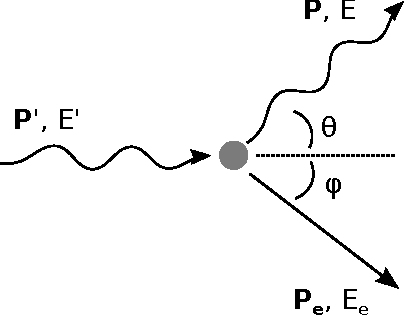
\includegraphics{backmatter/appendix_B/compton_scatter_free_electron.pdf}}
  \end{center}
  \caption{\textbf{Compton scattering off of a free electron.}}
  \label{fig:compton_scatter_free_electron}
\end{figure}

The process of Compton scattering off of a bound electron is represented by
figure \ref{fig:compton_scatter_bound_electron}.
\begin{figure}[t!]
  \begin{center}
    \scalebox{1.0}{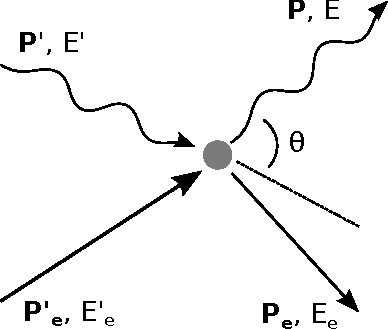
\includegraphics{backmatter/appendix_B/compton_scatter_bound_electron.pdf}}
  \end{center}
  \caption{\textbf{Compton scattering off of a bound electron.}}
  \label{fig:compton_scatter_bound_electron}
\end{figure}
Conservation of energy and momentum will again be used to determine the 
quantity of interest, which in this case is the initial electron momentum, 
$\vec{P_e^{'}}$, projected onto the photon scattering vector, 
$\vec{P} - \vec{P^{'}}$. The z-axis of the system will be set parallel to the
scattering vector. Therefore, the electron momentum projection will be 
represented by the variable $p_z$.

Before analyzing the energy of the particle system, then energy of the 
electron will be discussed. The kinetic energy of the electron will be
represented by, $E_{e,k}$.
\begin{align}
  E_e^2 & = m_e^2c^4 + P_e^2c^2 \nonumber \\
  & = \left(m_ec^2 + E_{e,k}\right)^2 \nonumber
\end{align}
\begin{equation}
  P_e^2c^2 = 2m_ec^2E_{e,k} + E_{e,k}^2
\end{equation}
The energy of the particle system is given below. The binding energy of the 
electron is $E_b$.
\begin{equation*}
  E^{'} + E_{e,k}^{'} + m_ec^2 = E + E_{e,k} + m_ec^2 + E_b
\end{equation*}
\begin{align}
  E^{'}-E-E_b & = E_{e,k} - E_{e,k}^{'} \nonumber \\
  \left(E^{'}-E-E_b\right)^2 & = \left(E_{e,k} - E_{e,k}^{'}\right)^2 \nonumber \\
  & = E_{e,k}^2 - 2E_{e,k}E_{e,k}^{'} + E_{e,k}^{'2} \nonumber \\
  & = P_e^2c^2 - 2m_ec^2E_{e,k} - 2E_{e,k}E_{e,k}^{'} + P_e^{'2}c^2 - 2m_ec^2E_{e,k}^{'}
  \nonumber \\
  & = \left(P_e^2 + P_e^{'2}\right)c^2 - 2m_ec^2E_{e,k}^{'} - 
  2E_{e,k}\left(m_ec^2 + E_{e,k}^{'}\right) \nonumber \\
  & = \left(P_e^2 + P_e^{'2}\right)c^2 - 2m_ec^2E_{e,k}^{'} - 
  2\left(E^{'}-E-E_b+E_{e,k}^{'}\right)\left(m_ec^2 + E_{e,k}^{'}\right) \nonumber\\
  & = \left(P_e^2 + P_e^{'2}\right)c^2 - 4m_ec^2E_{e,k}^{'} - 2E_{e,k}^{'2} -
  2\left(E^{'}-E-E_b\right)\left(m_ec^2 + E_{e,k}^{'}\right) \nonumber \\
  & = \left(P_e^2 - P_e^{'2}\right)c^2 -
  2\left(E^{'}-E-E_b\right)\left(m_ec^2 + E_{e,k}^{'}\right) \nonumber \\
  \left(P_e^2 - P_e^{'2}\right)c^2 & = \left(E^{'}-E-E_b\right)^2 +
  2\left(E^{'}-E-E_b\right)\left(m_ec^2 + E_{e,k}^{'}\right)
\end{align}

The momentum of the particle system will now be analyzed. 
\begin{align}
  \vec{P^{'}} + \vec{P_e^{'}} & = \vec{P} + \vec{P_e} \nonumber \\
  m_ec\vec{\alpha^{'}} + \vec{P_e^{'}} & = m_ec\vec{\alpha} + \vec{P_e} \nonumber
\end{align}
The new variable $\vec{\alpha}$ is simply the momentum of the photon in 
units of $m_ec$. The magnitude of this vector has the following properties.
\begin{align}
  \left|\vec{\alpha}\right| & = \alpha \nonumber \\
  & = \frac{P}{m_ec} \\ 
  & = \frac{E}{m_ec^2} 
\end{align}
The equation for the momentum of the system must be rearranged further before
moving on.
\begin{align}
  \vec{P_e^{'}} - \vec{P_e} & = \vec{q} \nonumber \\
  & = m_ec\left(\vec{\alpha} - \vec{\alpha^{'}}\right) \nonumber
\end{align}
\begin{align}
  q^2 & = (m_ec)^2\left|\vec{\alpha} - \vec{\alpha^{'}}\right| \nonumber \\
  & = (m_ec)^2\left(\alpha^{'2} + \alpha^2 - 
  2\vec{\alpha^{'}}\cdot\vec{\alpha}\right) \nonumber \\
  & = (m_ec)^2\left(\alpha^{'2} + \alpha^2 - 2\alpha^{'}\alpha\cos{\theta}\right)
\end{align}

Now, using the equation for $\vec{q}$, the equation for the electron momentum 
projection can be determined.
\begin{equation*}
  \vec{P_e} = \vec{P_e^{'}} - \vec{q}
\end{equation*}
\begin{equation*}
  P_e^2 = P_e^{'2} + q^2 - 2\vec{P_e^{'}}\cdot\vec{q}
\end{equation*}
\begin{equation*}
  2\vec{P_e^{'}}\cdot\vec{q} = -\left(P_e^2 - P_e^{'2}\right) + q^2
\end{equation*}
\begin{equation*}
  2p_zq = -\left(P_e^2 - P_e^{'2}\right) + q^2 \nonumber
\end{equation*}
\begin{align}
  p_z & = \frac{1}{2q}\left[-\left(P_e^2 - P_e^{'2}\right) + q^2\right] 
  \nonumber \\
  & = \frac{1}{2qc^2}\left[-(E^{'}-E-E_b)^2 - 2(E^{'}-E-E_b)(m_ec^2+E_{e,k}^{'})
    +q^2c^2\right] \nonumber \\
  & = \frac{m_e^2c^4}{2qc^2}\left[
    -\left(\alpha^{'}-\alpha-\frac{E_b}{m_ec^2}\right)^2 -
    2\left(\alpha^{'}-\alpha-\frac{E_b}{m_ec^2}\right)
    \left(1 + \frac{E_{e,k}^{'}}{m_ec^2}\right) + 
    \left|\vec{\alpha} - \vec{\alpha^{'}}\right|^2\right] \nonumber \\
  & = \frac{m_e^2c^2}{2q}\Bigg[-(\alpha^{'}-\alpha)^2 + 
    2(\alpha^{'}-\alpha)\left(\frac{E_b}{m_ec^2}\right) - 
    \left(\frac{E_b}{m_ec^2}\right)^2 -
    2(\alpha^{'}-\alpha)\left(1 + \frac{E_{e,k}^{'}}{m_ec^2}\right) + \nonumber \\
  & \qquad \qquad \qquad
    2\left(\frac{E_b}{m_ec^2}\right)\left(1 + \frac{E_{e,k}^{'}}{m_ec^2}\right) +
    \alpha^{'2} + \alpha^2 - 2\alpha^{'}\alpha\cos{\theta}\Bigg] \nonumber \\
  & = m_ec\frac{\left[(\alpha^{'}-\alpha)\left(1 + \frac{E_{e,k}^{'} - E_b}{m_ec^2}
    \right) + \alpha^{'}\alpha(1-\cos{\theta}) -
    \frac{1}{2}\left(\frac{E_b}{m_ec^2}\right)^2 + 
    \left(\frac{E_b}{m_ec^2}\right)\left(1 + \frac{E_{e,k}^{'}}{m_ec^2}\right)
    \right]} {\sqrt{\alpha^{'2} + \alpha^2 - 2\alpha^{'}\alpha\cos{\theta}}}
\end{align}
If the binding energy and kinetic energy of the electron are assumed to be 
small compared to the rest mass energy of the electron, they can be neglected. 
The resulting equation, which is often reported in the literature is the 
following.
\begin{equation}
  p_z = m_ec\frac{\left[\alpha - \alpha^{'} + \alpha^{'}\alpha(1-\cos{\theta})
      \right]}{\sqrt{\alpha^{'2} + \alpha^2 - 2\alpha^{'}\alpha\cos{\theta}}}
\end{equation}

Derivations that are similar to the ones just shown were completed by Sood
\citep{sood_doppler_2004}. 

\section{The Klein-Nishin Cross Section Differential in Inverse Energy Loss Ratio}
\label{diff_kn_cross_sec_var_change}
As mentioned in chapter \ref{ch:photon_interactions}, the differential 
Klein-Nishina cross section is most easily sampled when a change of variables
from steradians to the inverse energy loss ratio is conducted. The energy loss
ratio, which was originally shown in chapter \ref{ch:photon_interactions}, will
be shown again below.
\begin{align}
  \frac{1}{x} & = \frac{\alpha}{\alpha^{'}} \nonumber \\
  & = \frac{1}{1+\alpha^{'}(1-\cos{\theta})} \nonumber
\end{align}

The change of variables is conducted using the following relationship.
\begin{equation*}
  \frac{d\sigma_{K.N.}(\alpha^{'},x)}{dx} dx = 
  \frac{d\sigma_{K.N.}(\alpha^{'},\theta)}{d\Omega} d\Omega
\end{equation*}
\begin{equation*}
  \frac{d\sigma_{K.N.}(\alpha^{'},x)}{dx} = 
  \frac{d\sigma_{K.N.}(\alpha^{'},\theta)}{d\Omega}
  \left(\frac{d\Omega}{dx}\right)
\end{equation*}
Based on the equation for the energy loss ratio, the second term in the above
equation can be determined.
\begin{align}
  x = 1 + \alpha^{'}(1-\cos{\theta}) \nonumber \\
  dx = -\alpha^{'} d(\cos{\theta}) \nonumber
\end{align}
\begin{align}
  \frac{d\Omega}{dx} & = -2\pi\frac{d(\cos{\theta})}{dx} \nonumber \\
  & = \frac{2\pi}{\alpha^{'}}
\end{align}
The following relationships will also be useful while conducting the change
of variables.
\begin{align}
  x - 1 & = \alpha^{'}(1-\cos{\theta}) \\
  cos^2\theta & = 1 - \frac{2(x-1)}{\alpha^{'}} + \frac{(x-1)^2}{\alpha^{'2}}
\end{align}
Now, the change of variables can be completed.
\begin{align}
  \frac{d\sigma_{K.N.}(\alpha^{'},x)}{dx} & = \frac{r_e^2}{2}
  \frac{\left[1 + \cos{^{2}\theta} + \frac{\alpha^{'2}(1-\cos{\theta})^2}
                                  {1 + \alpha^{'}(1-\cos{\theta})}\right] }
  {\left[1 + \alpha^{'}(1-\cos{\theta}) \right]^2} 
  \left(\frac{2\pi}{\alpha^{'}}\right) \nonumber \\
  & = \left(\frac{\pi r_e^2}{\alpha^{'}x^2}\right)
  \left[1 + 
    \left(1 - \frac{2(x-1)}{\alpha^{'}} + \frac{(x-1)^2}{\alpha^{'2}}\right) +
    \frac{(x-1)^2}{x} \right] \nonumber \\
  & = \left(\frac{\pi r_e^2}{\alpha^{'}x^2}\right) \left[2 - 
    \frac{2x}{\alpha^{'}} + \frac{2}{\alpha^{'}} +\frac{x^2}{\alpha^{'2}} -
    \frac{2x}{\alpha^{'2}} + \frac{1}{\alpha^{'2}} + x - 2 + \frac{1}{x} \right]
  \nonumber \\
  & = \left(\frac{\pi r_e^2}{\alpha^{'}}\right) \left[ \frac{1}{\alpha^{'2}} +
    \frac{1}{x}\left(1 - \frac{2}{\alpha^{'}}-\frac{2}{\alpha^{'2}}\right) +
    \frac{1}{x^2}\left(\frac{2}{\alpha^{'}} + \frac{1}{\alpha^{'2}}\right) +
    \frac{1}{x^3} \right] \nonumber \\
  & = K \left[A + \frac{B}{x} + \frac{C}{x^2} + \frac{D}{x^3}\right]
\end{align}
\begin{align}
  K & = \frac{\pi r_e^2}{\alpha^{'}} \nonumber \\
  A & = \frac{1}{\alpha^{'}} \nonumber \\
  B & = 1 - \frac{2(\alpha^{'}+1)}{\alpha^{'2}} \nonumber \\
  C & = \frac{(1+2\alpha^{'})}{\alpha^{'2}} \nonumber \\
  D & = 1 \nonumber 
\end{align}

\section{The Total Klein-Nishina Cross Section}
Using the sampling methods from chapter \ref{ch:photon_interactions} will 
sometimes require the total Klein-Nishina cross section. Using the 
Klein-Nishina cross section differential in the inverse energy loss ratio,
the total Klein-Nishina cross section can be determined rather easily. The
integration of the differential cross section will be split up into four parts
and then recombined and reorganized to give the total cross section reported by 
Lux (with the error corrected) \citep{lux_monte_1991}. 
\begin{align}
  \sigma_{K.N.}(\alpha^{'}) & = \int_1^{1+2\alpha^{'}} \frac{d\sigma_{K.N.}(x)}{dx} dx
  \nonumber \\
  & = K \left(\int_1^{1+2\alpha^{'}} A dx + 
    \int_1^{1+2\alpha^{'}} \frac{B}{x} dx + 
    \int_1^{1+2\alpha^{'}} \frac{C}{x^2} dx + 
    \int_1^{1+2\alpha^{'}} \frac{D}{x^3} dx \right) \nonumber \\
  & = K \left(Ax \Bigg|_1^{1+2\alpha^{'}} + B\ln{x}\Bigg|_1^{1+2\alpha^{'}} -
    \frac{C}{x} \Bigg|_1^{1+2\alpha^{'}} - \frac{D}{2x^2} \Bigg|_1^{1+2\alpha^{'}}
    \right) \nonumber \\
  & = K \left(2\alpha^{'}A + B\ln{(1+2\alpha^{'})} - \frac{C}{1+2\alpha^{'}} + C -
    \frac{D}{2(1+2\alpha^{'})^2} + \frac{D}{2} \right) \nonumber \\
  & = K \left(\frac{2}{\alpha^{'}} + \ln{(1 + 2\alpha^{'})} -
    \frac{2(\alpha^{'}+1)}{\alpha^{'2}}\ln{(1+2\alpha^{'})} - 
    \frac{1}{\alpha^{'2}} + \frac{1+2\alpha^{'}}{\alpha^{'2}} - 
    \frac{1}{2(1+2\alpha^{'2})^2} + \frac{1}{2} \right) \nonumber \\
  & = K \left(\frac{2}{\alpha^{'}} + \ln{(1 + 2\alpha^{'})} -
    \frac{2(\alpha^{'}+1)}{\alpha^{'2}}\ln{(1+2\alpha^{'})} + 
    \frac{2}{\alpha^{'}} + \frac{2\alpha^{'}(1+\alpha^{'})}{(1+2\alpha^{'})^2} 
    \right) \nonumber \\
  & = K \left(\frac{4(1+\alpha^{'})^2}{\alpha^{'}(1+2\alpha^{'})} - 
      \frac{4\alpha^{'}}{1+2\alpha^{'}} + \ln{(1 + 2\alpha^{'})} -
    \frac{2(\alpha^{'}+1)}{\alpha^{'2}}\ln{(1+2\alpha^{'})} + 
    \frac{2\alpha^{'}(1+\alpha^{'})}{(1+2\alpha^{'})^2} 
    \right) \nonumber \\
  & = K \left(\frac{2(1+\alpha^{'})}{\alpha^{'}} 
    \left[\frac{2(1+\alpha^{'})}{1+2\alpha^{'}} - 
    \frac{\ln{(1+2\alpha^{'})}}{\alpha^{'}} \right] + \ln{(1 + 2\alpha^{'})} -
    \frac{4\alpha^{'}}{1+2\alpha^{'}} + 
    \frac{2\alpha^{'}(1+\alpha^{'})}{(1+2\alpha^{'})^2} \right) \nonumber \\
  & = K \left(\frac{2(1+\alpha^{'})}{\alpha^{'}} 
    \left[\frac{2(1+\alpha^{'})}{1+2\alpha^{'}} - 
    \frac{\ln{(1+2\alpha^{'})}}{\alpha^{'}} \right] + \ln{(1 + 2\alpha^{'})} -
    \frac{2\alpha^{'}(1+3\alpha^{'})}{(1+2\alpha^{'})^2} \right) \nonumber \\
  & = 2\pi r_e^2 \left(\frac{(1+\alpha^{'})}{\alpha^{'2}} 
    \left[\frac{2(1+\alpha^{'})}{1+2\alpha^{'}} - 
    \frac{\ln{(1+2\alpha^{'})}}{\alpha^{'}} \right] +
    \frac{\ln{(1 + 2\alpha^{'})}}{2\alpha^{'}} - 
    \frac{(1+3\alpha^{'})}{(1+2\alpha^{'})^2} \right) 
\end{align}

In the equation for the total Klein-Nishina cross section reported by Lux, the
second and third terms have an error \citep{lux_monte_1991}. The second term is
\begin{equation*}
  \frac{\ln{(1 + 2\alpha^{'})}}{2\alpha^{'}}.
\end{equation*}
In the equation reported by Lux, this term is
\begin{equation*}
  \frac{\ln{(1 + 2\alpha^{'})}}{2\alpha^{'2}}.
\end{equation*}
The third term is 
\begin{equation*}
  -\frac{(1+3\alpha^{'})}{(1+2\alpha^{'})^2}.
\end{equation*}
In the equation reported by Lux, this term is
\begin{equation*}
  -\frac{(1+3\alpha^{'})}{\alpha^{'}(1+2\alpha^{'})^2}.
\end{equation*}

\section{Kahn's Klein-Nishina Rejection Sampling Procedure}
\label{sec:Kahn_rejection_procedure_der}
As mentioned in chapter \ref{ch:photon_interactions}, below an incoming photon
energy of about 1.4 MeV, Kahn's rejection sampling procedure must be used to
sample the outgoing angle and energy of the photon after a Compton scattering
event. In this section, the derivation of this rejection sampling procedure will
be presented. First, rejection sampling must be explained. 

Most PDFs can be expanded in the following way.
\begin{equation}
  p(x) = \frac{\sum_i^m p_i T_i(x)n_i(x)}{\kappa}
  \label{eq:general_pdf_expansion}
\end{equation}
The number of factors, $m$, is arbitrary although splitting a PDF into more than
one factor can improve the sampling efficiency \citep{kahn_applications_1956}.
The probability of selecting a value of x from a particular factor is $p_i$.
The function $T_i(x)$ must be bounded in the interval (0,1). The efficiency
of the sampling procedure is $\kappa$. Now, to sample a value of $x$, one 
first samples an index $i$ from the disctrete PDF $p(i) = p_i$. Then, one 
samples a value of $x$ from the PDF $n_i(x)$. Finally, if the following 
equality holds, the value is accepted. Otherwise the entire process is repeated.
The quantity $\varepsilon$ is a uniform random number in the interval (0,1).
\begin{equation*}
  \varepsilon \leq T_i(x)
\end{equation*}

The simplest possible expansion for rejection sampling would be the following.
\begin{equation*}
  \kappa p(x) = \left(\frac{p(x)}{C}\right)\left(\frac{1}{b-a}\right)
\end{equation*}
Using this expansion, one would sample a value of x from the uniform 
distribution in the interval (a,b). Then the rejection function $\frac{p(x)}{C}$
would be used to determine if x should be accepted or rejected. The value of
C is simply the maximum value of the PDF $p(x)$.

Often, determining the expansion with the largest efficiency requires trial and
error as many possible expansions can exist for each PDF. This is the case with
the PDF corresponding to the differential Klein-Nishina cross section. Only the 
optimum expansion will be shown.

To begin, the PDF corresponding to the differential Klein-Nishina cross section 
will be derived. A change of variables to the inverse energy loss ratio must
be conducted first, which is shown in section 
\ref{diff_kn_cross_sec_var_change}.
\begin{equation*}
  \frac{d\sigma_{K.N.}(\alpha^{'},x)}{dx} = \frac{\pi r_e^2}{\alpha^{'}x^2}
  \left(\frac{1}{x} + x - 1 + cos^2\theta \right)
\end{equation*}
The PDF corresponding to this cross section is simply
\begin{align}
  p(\alpha^{'},x) & = 
  \begin{cases}
    \frac{1}{K(\alpha^{'})x^2}\left(\frac{1}{x} + x - 1 + cos^2\theta \right)
    & \text{if } 1 \leq x \leq 1 + 2\alpha^{'} \\
    0 & \text{o.w.}
  \end{cases} \\
  K(\alpha^{'}) & = \int_1^{1+2\alpha^{'}} \frac{dx}{x^2}
  \left(\frac{1}{x}+x-1+cos^2\theta \right) \nonumber \\
  & = \left(\frac{\alpha^{'}}{\pi r_e^2}\right) \sigma_{K.N}(\alpha^{'})
\end{align}

Now, the PDF will be factored into the following form.
\begin{equation*}
  \kappa p(\alpha^{'},x) = p_1(\alpha^{'})T_1(\alpha^{'},x)n_1(\alpha^{'},x) + 
  p_2(\alpha^{'})T_2(\alpha^{'},x)n_2(\alpha^{'},x)
\end{equation*}
The first factor $T_1(\alpha^{'},x)n_1(\alpha^{'},x)$ will have the following 
form.
\begin{equation*}
  T_1(\alpha^{'},x)n_1(\alpha^{'},x) = C_1(\alpha^{'})\left(\frac{1}{x} - 
  \frac{1}{x^2}\right)
\end{equation*}
The most efficient way to sample from this distribution is to sample a value
of x from the uniform distribution.
\begin{equation}
  n_1(\alpha^{'},x) = \frac{1}{2\alpha^{'}}
\end{equation}
The rejection function is then
\begin{equation*}
  T_1(\alpha^{'},x) = C_{T1}\left(\frac{1}{x} - \frac{1}{x^2}\right).
\end{equation*}
This function evaluates to zero when $x = 1$. The maximum value of this function
occurs when $x = 2$. Therefore, $C_{T1}$ must equal four so that the function
is always between zero and one.
\begin{equation}
  T_1(\alpha^{'},x) = 4\left(\frac{1}{x} - \frac{1}{x^2}\right).
\end{equation}

The second factor $T_2(\alpha^{'},x)n_2(\alpha^{'},x)$ will have the following 
form.
\begin{equation*}
  T_2(\alpha^{'},x)n_2(\alpha^{'},x) = \frac{C_2(\alpha^{'})}{x^2}
  \left(cos^2\theta + \frac{1}{x}\right)
\end{equation*}
The most efficienct way to sample from this distribution is to sample a value
of x from the follwing distribution.
\begin{equation}
  n_2(\alpha^{'},x) = \frac{1+2\alpha^{'}}{2\alpha^{'} x^2}
\end{equation}
The rejection function is then
\begin{equation*}
  T_2(\alpha^{'},x) = C_{T2}\left(cos^2\theta + \frac{1}{x} \right)
\end{equation*}
The maximum value of this function occurs when x equals unity and 
correspondingly, $\cos{\theta}$ equals unity. To ensure that this function is
always between zero and one, $C_{T2} = \frac{1}{2}$.
\begin{equation}
  T_2(\alpha^{'},x) = \frac{1}{2}\left(cos^2\theta + \frac{1}{x} \right)
\end{equation}

Now, the probabilities associated with each factor need to be determined.
\begin{equation*}
  \kappa p(\alpha^{'},x) = \frac{2 p_1(\alpha^{'})}{\alpha^{'}}
  \left(\frac{1}{x} - \frac{1}{x^2}\right) + 
  \frac{1+2\alpha^{'}}{4\alpha^{'}x^2}p_2 \left(cos^2\theta + \frac{1}{x}\right)
\end{equation*}
\begin{align}
  \frac{2p_1}{\alpha^{'}} & = \frac{1+2\alpha^{'}}{4\alpha^{'}}p_2 \nonumber \\
  & = \frac{1+2\alpha^{'}}{4\alpha^{'}}(1-p_1) \nonumber \\
  p_1\left(\frac{2}{\alpha^{'}} + \frac{1}{4\alpha^{'}} + \frac{1}{2} \right)
  & = \frac{1+2\alpha^{'}}{4\alpha^{'}} \nonumber \\
  p_1 = \frac{1+2\alpha^{'}}{9 + 2\alpha^{'}} \\
  p_2 = \frac{8}{9 + 2\alpha^{'}}
\end{align}
The efficiency associated with this rejection scheme is
\begin{equation}
  \kappa(\alpha^{'}) = \frac{2 K(\alpha^{'})(1+2\alpha^{'})}
  {\alpha^{'}(2\alpha^{'}+9)}.
\end{equation}

Kahn's rejection sampling procedure corresponds to the above expansion.
  
\section{The Adjoint Klein-Nishina Cross Section Differential in Inverse Energy Gain Ratio}
In this section, the derivation of the adjoint Klein-Nishina cross section
differential in inverse energy gain ratio will be shown. The energy gain
ratio, which was originally shown in chapter \ref{ch:photon_interactions}, 
will be shown again.
\begin{align}
  \frac{1}{x} & = \frac{\alpha}{\alpha^{'}} \nonumber \\
  & = \frac{1}{1 - \alpha^{'}(1-\cos{\theta})} \nonumber
\end{align}

The change of variables is conducted using the following relationship.
\begin{align}
  \frac{d\sigma_{K.N.}^{\dagger}(\alpha^{'},x)}{dx}dx & =
  \frac{d\sigma_{K.N.}^{\dagger}(\alpha^{'},\theta)}{dE}dE \nonumber \\
  \frac{d\sigma_{K.N.}^{\dagger}(\alpha^{'},x)}{dx} & = 
  \frac{d\sigma_{K.N.}^{\dagger}(\alpha^{'},\theta)}{dE} \left|\frac{dE}{dx}\right|
  \nonumber
\end{align}
Based on the equation for the energy gain ratio, the second term in the above
equation can be determined.
\begin{align}
  x = \frac{\alpha^{'}}{\alpha} \nonumber \\
  dx = -\frac{\alpha^{'}}{\alpha^2}d\alpha \nonumber
\end{align}
\begin{align}
  \frac{dx}{dE} & = -\frac{\alpha^{'}}{\alpha^2}\frac{d\alpha}{dE} \nonumber \\
  & = -\frac{\alpha^{'}}{m_ec^2\alpha^2}
\end{align}
The following relationship will also be useful while conducting the change
of variables.
\begin{equation}
  cos^2\theta = 1 - \frac{2(1-x)}{\alpha^{'}} + \frac{(1-x)^2}{\alpha^{'2}}
\end{equation}
Now the change of variables can be completed.
\begin{align}
  \frac{d\sigma_{K.N.}^{\dagger}(\alpha^{'},x)}{dx} & = 
  \frac{\pi r_e^2}{m_ec^2 \alpha^2}\left[x + \frac{1}{x} 
    - 1 + cos^2\theta \right] \left(\frac{m_ec^2\alpha^2}{\alpha^{'}}\right) 
  \nonumber \\
  & = \frac{\pi r_e^2}{\alpha^{'}} \left[x + \frac{1}{x} - 1 + cos^2\theta 
    \right] \\
  & = \frac{\pi r_e^2}{\alpha^{'}} \left[x + \frac{1}{x} - 1 + 1 - 
    \frac{2(1-x)}{\alpha^{'}} + \frac{(1-x)^2}{\alpha^{'2}} \right] \nonumber \\
  & = \frac{\pi r_e^2}{\alpha^{'}} \left[x + \frac{1}{x} - \frac{2}{\alpha^{'}} 
    + \frac{2x}{\alpha^{'}} + \frac{1}{\alpha^{'2}} - \frac{2x}{\alpha^{'2}} + 
    \frac{x^2}{\alpha^{'2}} \right] \nonumber \\
  & = \frac{\pi r_e^2}{\alpha^{'}} \left[\frac{1}{x} + 
    x\left(1 + \frac{2}{\alpha^{'}} - \frac{2}{\alpha^{'2}}\right) +
    x^2\left(\frac{1}{\alpha^{'2}}\right) - \frac{2}{\alpha^{'}} + 
    \frac{1}{\alpha^{'2}} \right] \nonumber \\
  & = K^{\dagger}\left[A^{\dagger}x^2 + B^{\dagger}x + C^{\dagger} + 
    \frac{D^{\dagger}}{x} \right]
\end{align}
\begin{align}
  K^{\dagger} & = \frac{\pi r_e^2}{\alpha^{'}} \nonumber \\
  A^{\dagger} & = \frac{1}{\alpha^{'2}} \nonumber \\
  B^{\dagger} & = 1 + \frac{2(\alpha^{'}-1)}{\alpha^{'2}} \nonumber \\
  C^{\dagger} & = \frac{1-2\alpha^{'}}{\alpha^{'2}} \nonumber \\
  D^{\dagger} & = 1 \nonumber
\end{align}
  
\section{Efficient Adjoint Klein-Nishina Rejection Sampling Procedure}
As explained in section \ref{sec:Kahn_rejection_procedure_der} and shown in
equation \ref{eq:general_pdf_expansion}, a PDF can be split into many factors 
from which values of the PDF are sampled. In the case of the PDF corresponding 
to the differential adjoint Klein-Nishina cross section, three factors will 
used. 
\begin{align}
  \kappa p_{K.N.}^{\dagger}(x|\alpha^{'},\alpha_{max}) & = 
  p_1(\alpha^{'},\alpha_{max})T_1(\alpha^{'},\alpha_{max},x)
  n_1(\alpha^{'},\alpha_{max},x) \nonumber \\
  & \quad + p_2(\alpha^{'},\alpha_{max})T_2(\alpha^{'},\alpha_{max},x)
  n_2(\alpha^{'},\alpha_{max},x) \nonumber \\
  & \quad + p_3(\alpha^{'},\alpha_{max})T_3(\alpha^{'},\alpha_{max},x)
  n_3(\alpha^{'},\alpha_{max},x) \nonumber 
\end{align}
The PDF corresponding to the differential adjoint Klein-Nishina cross section 
was shown in equation \ref{eq:reorganized_adjoint_KN_pdf}. It will be shown 
here again for convenience.
\begin{equation}
  p_{K.N.}^{\dagger}(x|\alpha^{'},\alpha_{max}) = 
  \begin{cases}
    H^{\dagger}\left[\left(\frac{1}{x} - 1 \right) + \left(x\right) + 
      \left(cos^2\theta\right) \right] 
    & \text{if } x_{min} \leq x \leq 1 \\
    0 & \text{o.w.}
  \end{cases}
\end{equation}
The three terms from which the three factors will be derived are shown in
parenthesis in the above equation. 

The first factor $T_1(\alpha^{'},\alpha_{max},x)n_1(\alpha^{'},\alpha_{max},x)$
will have the following form.
\begin{equation*}
  T_1(\alpha^{'},\alpha_{max},x)n_1(\alpha^{'},\alpha_{max},x) = 
  C_1(\alpha^{'},\alpha_{max})\left(\frac{1}{x}-1\right)
\end{equation*}
The most efficient way to sample from this distribution is to sample a value of
x from the following distribution.
\begin{equation}
  n_1(\alpha^{'},\alpha_{max},x) = -\frac{1}{x\ln{x_{min}}}
\end{equation}
The rejection function is then 
\begin{equation*}
  T_1(\alpha^{'},\alpha_{max},x) = C_{T1}(\alpha^{'},\alpha_{max})(1-x).
\end{equation*}
This function evaluates to zero when $x=1$. The maximum value of this function
occurs when $x=x_{min}$. Therefore, this function must be defined as follows.
\begin{equation}
  T_1(\alpha^{'},\alpha_{max},x) = \frac{1-x}{1-x_{min}}
\end{equation}

The second factor $T_2(\alpha^{'},\alpha_{max},x)n_2(\alpha^{'},\alpha_{max},x)$
will have the following form.
\begin{equation*}
  T_2(\alpha^{'},\alpha_{max},x)n_2(\alpha^{'},\alpha_{max},x) = 
  C_2(\alpha^{'},\alpha_{max})x
\end{equation*}
This distribution can be sampled from directly. Therefore a value of x will
be sampled from the following distribution.
\begin{equation}
  n_2(\alpha^{'},\alpha_{max},x) = \frac{2x}{1-x_{min}^2}
\end{equation}
The rejection function is then simply unity due to the direct sampling.

The third factor $T_3(\alpha^{'},\alpha_{max},x)n_3(\alpha^{'},\alpha_{max},x)$
will have the following form.
\begin{align}
  T_3(\alpha^{'},\alpha_{max},x)n_3(\alpha^{'},\alpha_{max},x) & = 
  C_3(\alpha^{'},\alpha_{max})cos^2\theta \nonumber \\
  & = C_3(\alpha^{'},\alpha_{max})
  \left(1 - \frac{1}{\alpha^{'}} + \frac{x}{\alpha^{'}}\right)^2 \nonumber \\
  & = \frac{C_3(\alpha^{'},\alpha_{max})}{\alpha^{'2}}\left(x-1+\alpha^{'}\right)^2
  \nonumber \\
\end{align}
This distribution can also be sampled from directly. Therefore a value of x
will be sampled from the following distribution.
\begin{equation}
  n_3(\alpha^{'},\alpha_{max},x) = \frac{3\left(x-1+\alpha^{'}\right)^2}
  {\alpha^{'3} - \left(x_{min}-1+\alpha^{'}\right)^3}
\end{equation}
The rejection function will again be simply unity due to the direct sampling.

Now the probabilities associated with each factor need to be determined.
\begin{align}
  \kappa p_{K.N.}^{\dagger}(x|\alpha^{'},\alpha_{max}) & = 
  -\frac{p_1(\alpha^{'},\alpha_{max})}{x\ln{x_{min}}}
  \left(\frac{1-x}{1-x_{min}}\right) +
  \frac{2xp_2(\alpha^{'},\alpha_{max})}{1-x_{min}^2} \nonumber \\
  & \quad +
  \frac{3p_3(\alpha^{'},\alpha_{max})\left(x-1+\alpha^{'}\right)^2}
  {\alpha^{'3} - \left(x_{min}-1+\alpha^{'}\right)^3} \nonumber
\end{align}

\begin{align}
  \frac{2p_2(\alpha^{'},\alpha_{max})}{1-x_{min}^2} & = 
  -\frac{p_1(\alpha^{'},\alpha_{max})}{\ln{x_{min}}\left(1-x_{min}\right)} \\
  \frac{2p_2(\alpha^{'},\alpha_{max})}{1-x_{min}^2} & = 
  \frac{3\alpha^{'2}p_3(\alpha^{'},\alpha_{max})}
       {\alpha^{'3} - \left(x_{min}-1+\alpha^{'}\right)^3} \\
  1 = p_1(\alpha^{'},\alpha_{max}) & + p_2(\alpha^{'},\alpha_{max}) +
  p_3(\alpha^{'},\alpha_{max})
\end{align}
By solving the above system of equations, the probabilities can be determined, 
which are shown below.
\begin{align}
  p_1(\alpha^{'},\alpha_{max}) & = 
  -\frac{3\ln{x_{min}}\left(1-x_{min}\right)\alpha^{'2}}
  {\frac{3}{2}\left(1-x_{min}^2\right)\alpha^{'2} - 
    3\ln{x_{min}}\left(1-x_{min}\right)\alpha^{'2} + \alpha^{'3} - 
    \left(x_{min}-1+\alpha^{'}\right)^3} \\
  p_2(\alpha^{'},\alpha_{max}) & = 
  \frac{\frac{3}{2}\left(1-x_{min}^2\right)\alpha^{'2}}
  {\frac{3}{2}\left(1-x_{min}^2\right)\alpha^{'2} - 
    3\ln{x_{min}}\left(1-x_{min}\right)\alpha^{'2} + \alpha^{'3} - 
    \left(x_{min}-1+\alpha^{'}\right)^3} \\
  p_3(\alpha^{'},\alpha_{max}) & =
  \frac{\alpha^{'3} - \left(x_{min}-1+\alpha^{'}\right)^3}
  {\frac{3}{2}\left(1-x_{min}^2\right)\alpha^{'2} - 
    3\ln{x_{min}}\left(1-x_{min}\right)\alpha^{'2} + \alpha^{'3} - 
    \left(x_{min}-1+\alpha^{'}\right)^3}
\end{align}
The efficiency associated with this rejection scheme is 
\begin{align}
  \kappa(\alpha^{'}&,\alpha_{max}) = 
  \frac{\alpha^{'}\sigma_{K.N.}^{\dagger}(\alpha^{'},\alpha_{max})}{\pi r_e^2}
  \nonumber \\
  &\cdot \left(\frac{3\alpha^{'2}}{\frac{3}{2}\left(1-x_{min}^2\right)\alpha^{'2} 
    -3\ln{x_{min}}\left(1-x_{min}\right)\alpha^{'2} + \alpha^{'3} - 
    \left(x_{min}-1+\alpha^{'}\right)^3}\right)
\end{align}
  
